\documentclass{article}
\usepackage{amsmath}
\usepackage{mathtools}
\usepackage{txfonts}
\usepackage{titlesec}
\usepackage[margin=0.5in]{geometry}
\usepackage{pdfpages}

\setlength{\parskip}{\baselineskip}%
\setlength{\parindent}{0pt}%

\title{Homework 2}
\author{Daniel Hartig}


\begin{document}
\maketitle

\titlespacing{\subsection}{0pt}{0pt}{0pt}
\titlespacing{\subsubsection}{0pt}{0pt}{-\parskip}

\subsection*{Problem 3.3}
\subsubsection*{a., b., c.}
For a 95\% confidence interval, $\alpha/2 = 0.025$ and $z_{\alpha/2} = -1.960$. 
\begin{align*}
\log\hat{\theta} &= \log\left(\frac{60(61)}{2(44)}\right) = 3.728 \\
\hat{\sigma}\left(\log\hat{\theta}\right) &= \sqrt{\frac{1}{60} + \frac{1}{61} + \frac{1}{2} + \frac{1}{44}} = .746\\ 
\log \hat{\theta} \pm z_{\alpha/2}\hat{\sigma}\left(\log\hat{\theta}\right) &=3.728 \pm 1.960(0.746) = (2.267,5.189)  \\
\text{Confidence Interval}[\hat{\theta}] &= (e^{2.267}, e^{5.189}) = (9.648, 179.299)
\end{align*}
The main factor causing the confidence interval to be so large is the sample of two in the category of "Strong Republican, Strong Agree." In the calculation of standard error, it can be seen that the term $1/2$ dominates within the square root.

\subsection*{Problem 3.4}
\subsubsection*{a. Odds Ratio}
\begin{align*}
\log \hat{\theta} &= \log\left(\frac{1085(441239)}{703(55623)}\right) = 2.505 \\
\hat{\sigma}\left(\log\hat{\theta}\right) &= \sqrt{\frac{1}{1085}+\frac{1}{55623}+\frac{1}{703}+\frac{1}{441239}} = 0.0486 \\
\log \hat{\theta} \pm z_{\alpha/2}\hat{\sigma}\left(\log\hat{\theta}\right) &= 2.505 \pm 1.960(0.0486) = (2.464, 2.546) \\
\text{Confidence Interval}[\hat{\theta}] &= (e^{2.464}, e^{2.546}) = (11.756, 12.751)
\end{align*}
A driver or passenger involved in an auto accident is between 11.8 and 12.8 times more likely to become a fatality if that person is not wearing a seat-belt compared to if that person is wearing a seat belt. 
\subsubsection*{b. Difference of Proportions}
Let $\hat\pi_{no}$ be the probability of a fatality for a driver or passenger not using a seat-belt and $\hat\pi_{yes}$ be the probability if using a seat-belt.
\begin{align*}
\hat\pi_{no} &= \frac{y_{no}}{n_{no}} = \frac{1085}{1085+55623} =  0.0191 \\
\hat\pi_{yes} &= \frac{y_{yes}}{n_{yes}} = \frac{703}{703+441239} = 0.00159 \\
\hat\pi_{no} - \hat\pi_{yes} &= 0.0191 - 0.00159 = 0.0175 \\
\hat\sigma\left(\hat\pi_{no} - \hat\pi_{yes}\right) &=  \sqrt{\frac{\hat\pi_{no}(1-\hat\pi_{no})}{n_{no}} + \frac{\hat\pi_{no}(1-\hat\pi_{no})}{n_{no}}} = \sqrt{\frac{0.0191(1-0.0191)}{55623}+\frac{0.00159(1-.00159)}{441239}} = 0.000584 \\
\text{Confidence Interval}[\hat\pi_{no} - \hat\pi_{yes}] &= \hat\pi_{no} - \hat\pi_{yes} \pm z_{\alpha/2}\hat\sigma\left(\hat\pi_{no} - \hat\pi_{yes}\right) = 0.0175 \pm 1.960(0.000584) = (0.0164, 0.0187)
\end{align*}
A driver or passenger involved in an auto accident is between 1.6 and 1.9 percentage points more likely to become a fatality if that person is not wearing a seat-belt compared to if that person is wearing a seat belt.
\subsubsection*{c. Relative Risk}
\begin{align*}
\log r &= \log\left(\frac{\hat\pi_{no}}{\hat\pi_{yes}}\right) = \log\left(\frac{0.0191}{0.00159}\right) = 2.487 \\
\hat\sigma\left(\log r\right) &= \sqrt{\frac{1-\hat\pi_{no}}{y_{no}} + \frac{1-\hat\pi_{yes}}{y_{yes}}} = \sqrt{\frac{1-.0191}{1085}+\frac{1-.00159}{703}} = 0.0482 \\
\log r \pm z_{\alpha/2}\hat\sigma\left(\log r\right) &= 2.505 \pm 1.960 (0.0482) = (2.410, 2.599) \\
\text{Confidence Interval}[r] &= (e^{2.410}, e^{2.599}) = (10.943, 13.220)
\end{align*}
A driver of passenger involved in an auto accident is between 10.9 and 13.2 times more likely to become a fatality if that person is not wearing a seat belt compared to all people involved in car accidents. The reason this number is so close to the values obtained in the Odds Ratio confidence interval is that the probability of becoming a fatality is low, so the number of non-fatal accidents and the number of total accidents are close. 

\subsection{Problem 3.9}
The 2014 edition of the GSS yielded the following table for the variables "EDUCATION" and "FUND"
\begin{center}
\begin{tabular}{l c c c r}
&Fundamentalist&Moderate&Liberal&Row Total \\
K-12&307&461&270&1038 \\
13-18&262&508&472&1242 \\
19 or greater&16&56&69&141 \\
Column Total&585&1025&811&2421 
\end{tabular}
\end{center}
Solved using python 3.5 code attached at end of assignment. 
\subsubsection{a.}
The $X^2$ statistic is 63.822 with p-value $4.556\times10^{-13}$. The $G^2$ statistic is 65.443 with p-value $2.075\times10^{-13}$. There are 4 degrees of freedom. Because of the very high p-values, we have very high confidence that education and fundamentalism are not independent variables. 
\subsubsection{b.} 
There is a clear relationship between the fundamentalist and liberal positions and having or not having a college education. The number of fundamentalists with no college education is 5.39 standard deviations above expected, while the number of  fundamentalists with a college education is 3.62 stdev below expected and graduate school is 3.66 stdev below expected. Conversely, the number of liberals with no college education is 6.76 stdev lower than expected while the number of liberals with a college education is 4.81 stdev above expected and grad school is 4.00 stdev above expected.

The moderate position has a similar relationship to education as the fundamentalist, but this relationship is weaker. There is limited difference in the ideologies of those people who have been to college, and those who have been to graduate school. Overall, the significant finding is that fundamentalism is more likely in those without college education and liberalism is more likely in those with college education. 

\subsection{Problem 3.31}
\subsubsection{a.}
For the given table, the marginal distributions in both directions for the given table are 
\begin{align*}
\pi_{1+} &= \pi_{+1} = \theta^2 + \theta(1-\theta) = \theta \\
\pi_{2+} &= \pi_{+2} = (1-\theta)^2 + \theta(1-\theta) = 1-\theta \\
\end{align*}
so that the resulting table with marginals is 
\begin{center}
\begin{tabular}{lccc}
&Success in $j$&Failure in $j$&Marginal in $j$\\
Success in $i$&$\theta^2$&$\theta(1-\theta)$&$\theta$ \\ 
Failure in $i$&$\theta(1-\theta)$&$(1-\theta)^2$&$(1-\theta)$ \\ 
Marginal in $i$&$\theta$&$(1-\theta)$&1 \\
\end{tabular}
\end{center}
To prove independence, we calculate $\pi_{ij}$ from the marginals for all entries of the table and verify that we see the expected values in the table.
\begin{align*}
\pi_{11} &= \theta^2 = \theta(\theta) = \pi_{1+}\pi_{+1} \\
\pi_{12} = \pi_{21} &= \theta(1-\theta) = \pi{1+}\pi{+2} = \pi{+1}\pi{2+} \\
\pi_{22} &= (1-\theta)^2 = (1-\theta)(1-\theta)= \pi_{2+}\pi_{+2}
\end{align*}
\subsubsection{b.}
Since $\hat\theta$ represents the overall proportion of expected successes of either trial $i$ or trial $j$, it is represented by 
\begin{align*}
\hat\theta &= \frac{\hat n_1 + \hat n_2}{\hat n + \hat n} = \frac{1}{2}\left(\pi_1 + \pi_2\right) \\
&= \frac{\pi_{1+}+\pi_{+1}}{2}
\end{align*}


\subsubsection{c.}
To test a null hypothesis of independence, we use the Chi Squared test. The test statistic is 
\[\chi^2 = \sum_{i}\sum_{j}\frac{\left(n_{ij}-E(n_{ij})\right)^2}{E(n_{ij})}\]
If we divide through by $n$, the unknown sample size, we obtain an expression in terms of sample and expected proportions
\[\chi^2 = \sum_{i}\sum_{j}\frac{\left(\pi_{ij}-\hat\pi_{ij}\right)^2}{\hat\pi_{ij}}.\]
The degrees of freedom of a test of $H_0$ are $(I-1) + (J-1) = (2-1) + (2-1) = 2$. We expect the two degrees of freedom because the table is symmetrical in addition to being independent.
We then find a p-value for the obtained test statistic with the given degrees of freedom and use our desired confidence level to determine whether or not to reject $H_0$.

\subsubsection{d.}
The contingency table of sampled shots in its proportional form is
\begin{center}
\begin{tabular}{lcc|c}
&Made 2nd&Missed 2nd&\\
Made 1st&0.661&0.143&0.804 \\ 
Missed 1st&0.161&0.035&0.196 \\ \hline
&0.822&0.178&1 \\ 
\end{tabular}
\end{center}
The overall proportion of shots made is $0.813$, which is $\hat\theta$. Therefore, the expected shots table in proportional form is
\begin{center}
\begin{tabular}{lcc|c}
&Made 2nd&Missed 2nd&\\
Made 1st&0.661&0.152&0.813 \\ 
Missed 1st&0.152&0.035&0.187 \\ \hline
&0.813&0.187&1 \\ 
\end{tabular}
\end{center}
The chi squared test statistic is
\begin{align*}
\chi^2 &= \frac{(0.661-0.661)^2}{0.661} + \frac{(0.143-0.152)^2}{0.152} + \frac{(0.161-0.152)^2}{0.152} + \frac{(0.035-0.035)^2}{0.035} \\
&=4.379\times10^{-8} + 4.782\times10^{-4} + 5.171\times10^{-4} + 8.281\times10^{-7} \\
&= 0.000996
\end{align*}
Since the p-value is so low we cannot reject the null hypothesis. It is very plausible that Kobe Bryant's free throws are both independent and identically distributed. 

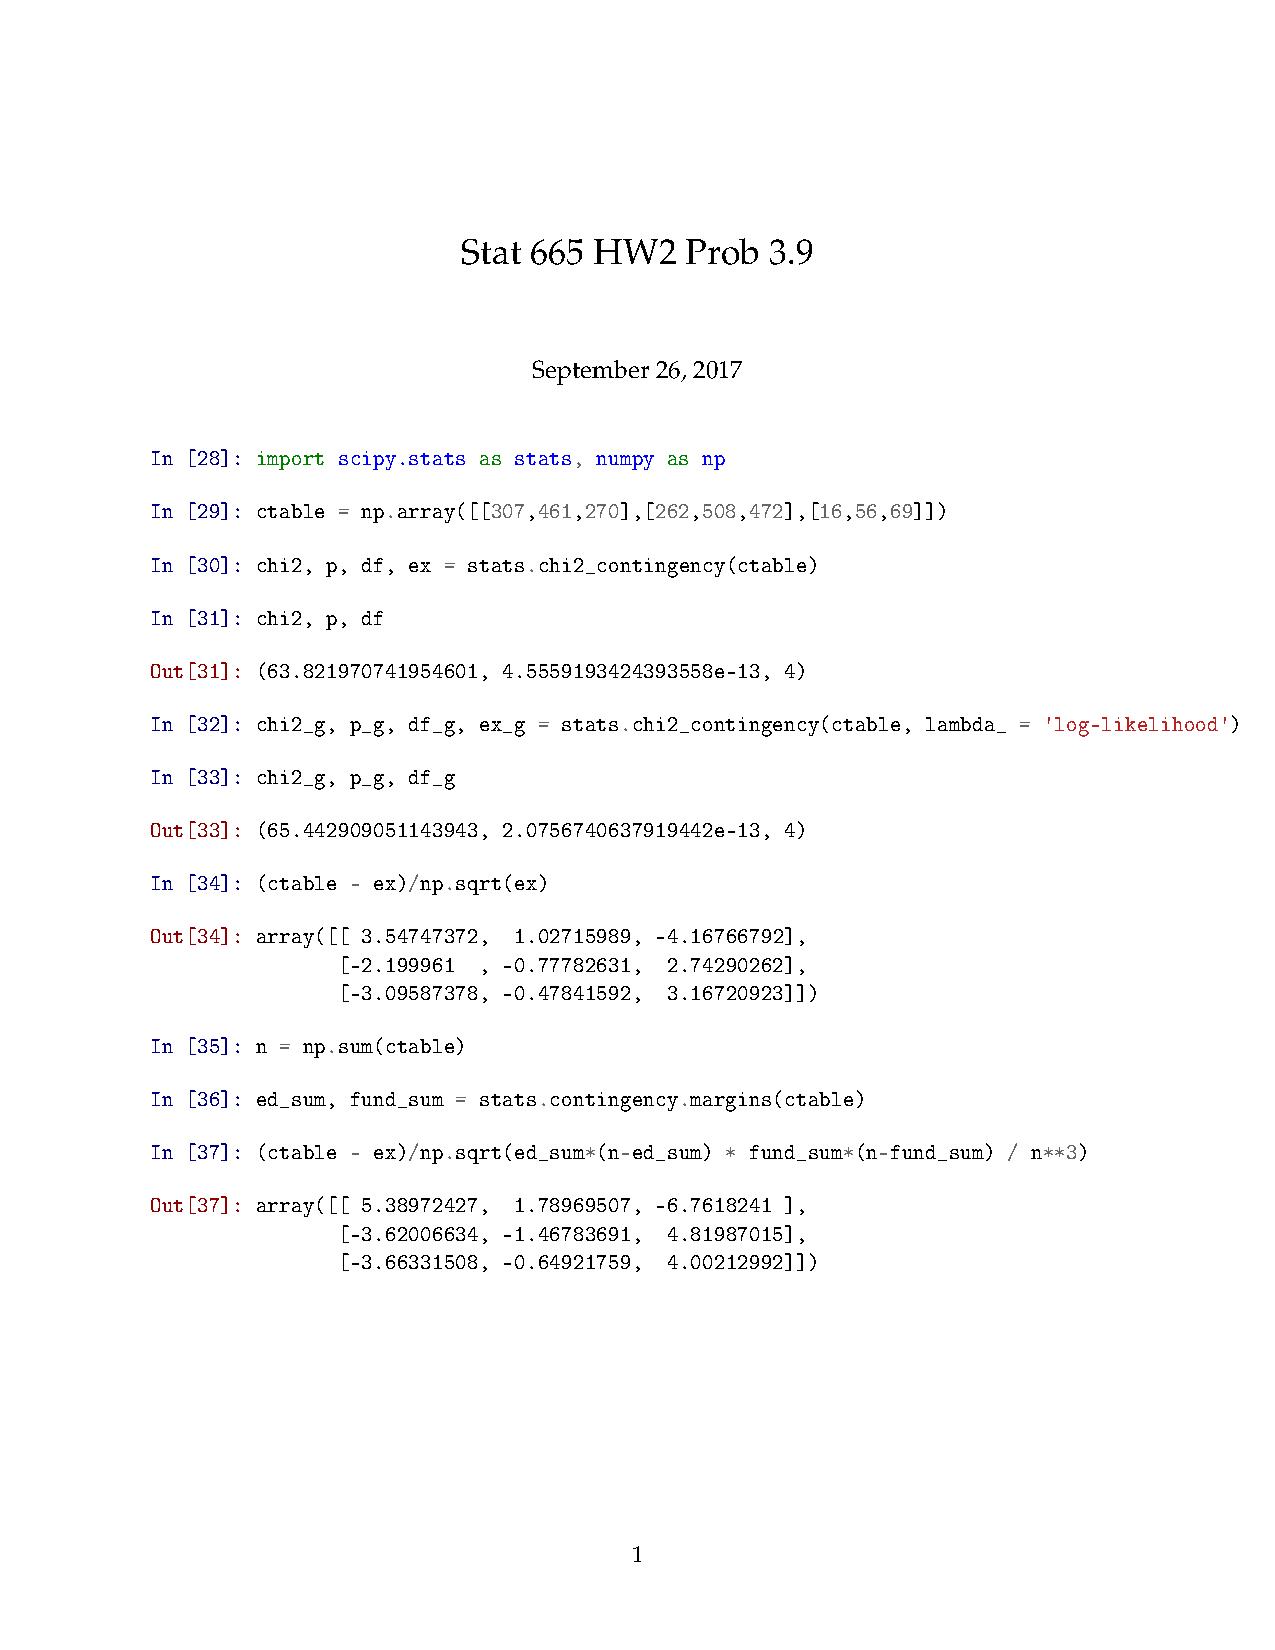
\includepdf{Stat+665+HW2+Prob+3_9.pdf}






\end{document}